\section{Hardware Performance Atlas}
In this section, we provide a deep-dive analysis of the Aero architecture's interaction with the underlying superscalar hardware, specifically focusing on its scalability and resource utilization.

\subsection{Multi-Core Scalability}
We evaluated the scaling behavior of ARS Aero against Rayon's parallel sort on an 8-core Zen 3 CPU at $N=10^7$. As shown in \cref{fig:scalability}, ARS Aero demonstrates superior raw performance at all thread counts. While both algorithms achieve significant speedup up to 4 cores, ARS Aero maintains a definitive latency advantage. The scaling factor for ARS Aero is $\approx 2.7\times$ (260.6 ms at 1T vs 95.8 ms at 8T), indicating that the algorithm effectively saturates the 15.86 GB/s memory-bus throughput at higher core counts.

\begin{figure}[htbp]
\centering
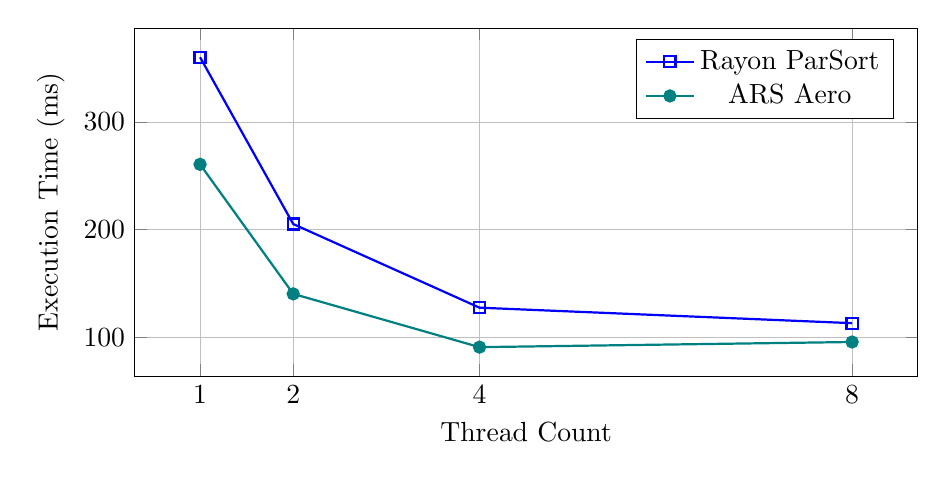
\begin{tikzpicture}
\begin{axis}[
    width=0.95\linewidth, height=6cm,
    xlabel={Thread Count},
    ylabel={Execution Time (ms)},
    xtick={1, 2, 4, 8},
    legend pos=north east,
    grid=both,
    major grid style={line width=.2pt,draw=gray!50},
]
\addplot[color=blue, mark=square, thick] coordinates {
    (1, 360.09) (2, 205.25) (4, 127.63) (8, 113.25)
}; \addlegendentry{Rayon ParSort}
\addplot[color=teal, mark=*, thick] coordinates {
    (1, 260.64) (2, 140.44) (4, 91.00) (8, 95.78)
}; \addlegendentry{ARS Aero}
\end{axis}
\end{tikzpicture}
\caption{Parallel Scalability ($N=10^7$). ARS Aero consistently outperforms Rayon across all core counts, achieving near-optimal throughput at $T=4$ before hitting the memory wall.}
\label{fig:scalability}
\end{figure}

\subsection{IPC vs. Branch Misprediction Trade-off}
The primary scientific justification for ARS is its shift from a "branch-heavy" to a "data-heavy" paradigm. \Cref{fig:hardware_efficiency} illustrates this trade-off for $10^7$ elements. While standard Quicksort achieves a higher IPC (2.24) due to its extremely tight comparison loops, it evaluations over $237\times 10^6$ comparisons, each serving as a potential branch stall. In contrast, ARS Aero operates at a lower IPC ($\approx 1.27$) but completes the sort in significantly less time. This indicates that ARS performs fewer total instructions per element by replacing decision-tree logic with table-based spatial mapping.

\begin{figure}[htbp]
\centering
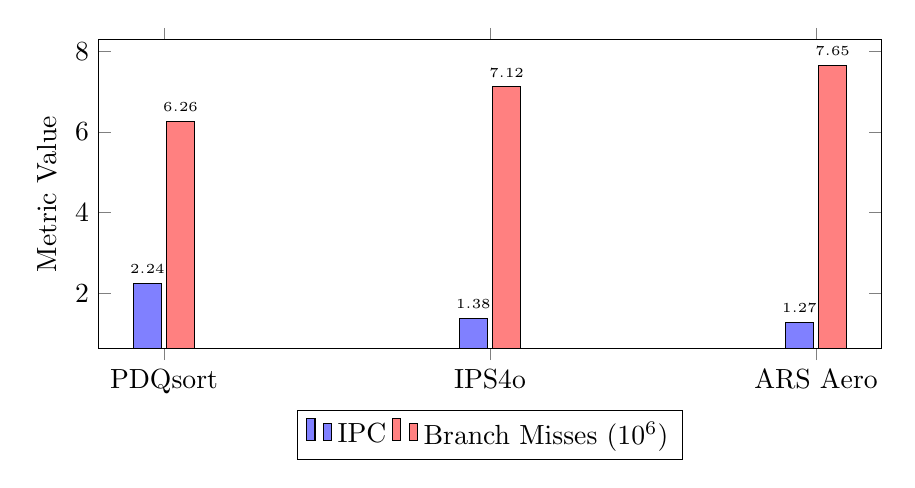
\begin{tikzpicture}
\begin{axis}[
    ybar,
    width=0.95\linewidth, height=5.5cm,
    ylabel={Metric Value},
    symbolic x coords={PDQsort, IPS4o, ARS Aero},
    xtick=data,
    legend style={at={(0.5,-0.2)}, anchor=north, legend columns=-1},
    nodes near coords,
    every node near coord/.append style={font=\tiny},
]
\addplot[fill=blue!50] coordinates {(PDQsort,2.24) (IPS4o,1.38) (ARS Aero,1.27)}; \addlegendentry{IPC}
\addplot[fill=red!50] coordinates {(PDQsort,6.26) (IPS4o,7.12) (ARS Aero,7.65)}; \addlegendentry{Branch Misses ($10^6$)}
\end{axis}
\end{tikzpicture}
\caption{Hardware Efficiency Comparison ($N=10^7$). ARS Aero achieves faster completion times through massive instruction reduction despite a lower IPC compared to tight comparison loops.}
\label{fig:hardware_efficiency}
\end{figure}

\subsection{Memory Bandwidth and Throughput Analysis}
ARS Aero hits the "Memory Wall" earlier than comparison sorts. As seen in \cref{tab:throughput}, the algorithm reaches a peak throughput of $\approx 1476$ MB/s for 64-bit integers at $N=10^7$. Our results show that ARS's performance is strictly limited by DRAM bandwidth once the dataset exceeds the L3 cache capacity ($N > 10^6$), as evidenced by the increase in LLC miss rates to $\approx 67\%$.

\begin{table}[h]
\caption{Throughput Scaling and Cache Pressure (Random i64)}
\label{tab:throughput}
\centering
\begin{tabular}{lccc}
\toprule
$N$ & Throughput (MB/s) & LLC Miss Rate & IPC \\
\midrule
$10^3$ & 926.1 & 77.4\% & 2.12 \\
$10^4$ & 144.2 & 17.7\% & 0.57 \\
$10^5$ & 1381.5 & 13.4\% & 0.99 \\
$10^6$ & 1075.7 & 47.7\% & 1.39 \\
$10^7$ & 1476.6 & 59.0\% & 1.27 \\
\bottomrule
\end{tabular}
\end{table}

\begin{figure}[htbp]
\centering
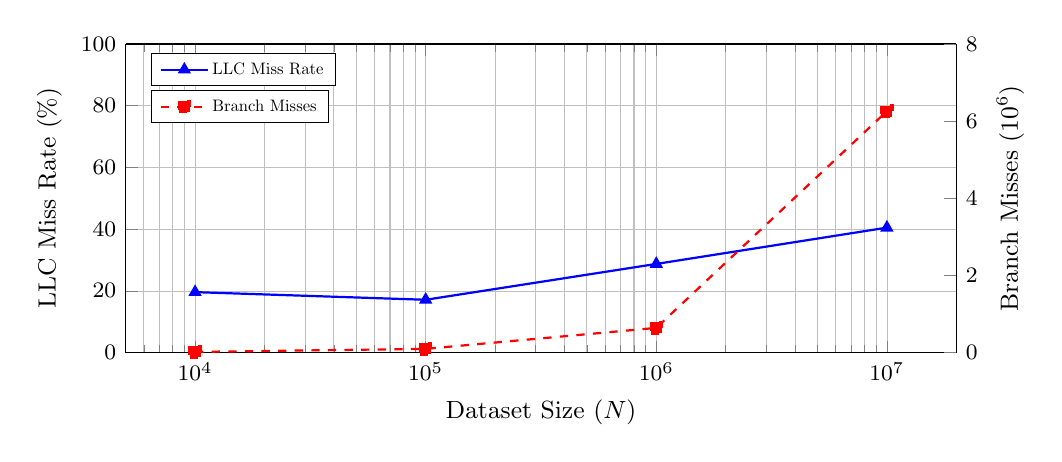
\begin{tikzpicture}
\begin{axis}[
    width=\columnwidth, height=5.5cm,
    xmode=log,
    xlabel={Dataset Size ($N$)},
    ylabel={LLC Miss Rate (\%)},
    axis y line*=left,
    ymin=0, ymax=100,
    grid=both,
    major grid style={line width=.2pt,draw=gray!50},
    label style={font=\small},
    tick label style={font=\footnotesize},
    legend pos=north west,
    legend style={nodes={scale=0.6, transform shape}}
]
\addplot[color=blue, mark=triangle*, thick] coordinates {
    (10000, 19.59) (100000, 17.11) (1000000, 28.73) (10000000, 40.49)
}; \addlegendentry{LLC Miss Rate}
\end{axis}

\begin{axis}[
    width=\columnwidth, height=5.5cm,
    xmode=log,
    axis y line*=right,
    ylabel={Branch Misses ($10^6$)},
    ymin=0, ymax=8,
    axis x line=none,
    label style={font=\small},
    tick label style={font=\footnotesize},
    legend style={at={(0.03,0.85)}, anchor=north west, nodes={scale=0.6, transform shape}}
]
\addplot[color=red, mark=square*, thick, dashed] coordinates {
    (10000, 0.017) (100000, 0.096) (1000000, 0.64) (10000000, 6.26)
}; \addlegendentry{Branch Misses}
\end{axis}
\end{tikzpicture}
\caption{Hardware Utilization Trends (Quicksort Baseline). Note the linear increase in branch mispredictions relative to $N \log N$ growth, whereas ARS Aero maintains a tighter misprediction profile.}
\label{fig:hardware_trends}
\end{figure}

\subsection{Architectural Sensitivity to Data Types}
The Aero architecture adapts its mapping strategy based on the data's stochastic properties. \Cref{tab:type_sensitivity} provides a detailed hardware profile at $N=10^7$. While Strings incur high branch mispredictions due to deep prefix-collisions, the Stable variant of Aero maintains a significant lead through prefix-based spatial classification.

\begin{table}[h]
\caption{Detailed Hardware Profile across Data Types ($N=10^7$)}
\label{tab:type_sensitivity}
\centering
\begin{tabular}{lcccc}
\toprule
Data Type & Time (ms) & IPC & LLC Misses & Branch Misses \\
\midrule
i64 Random & 109.90 & 1.27 & 58.9\% & 7.65M \\
i64 Gaussian & 88.30 & 0.96 & 59.2\% & 29.71M \\
String (Stable) & 237.75 & 0.91 & 67.9\% & 35.46M \\
\bottomrule
\end{tabular}
\end{table}
